\subsubsection{Stanford Arm}

Los brazos robóticos han sido un gran pilar en el desarrollo de la tecnología por su gran utilidad. Actualmente rara es la fábrica que no emplea brazos robóticos para hacer la producción mucho más ágil e incluso segura para los operadores de la misma. Este camino fue iniciado en el año 1969 en la Universidad de Stanford por Victor Scheinman.

\vspace{10px}

El primer brazo robótico fue desarrollado bajo el proyecto Hand-Eye en los laboratorios de Inteligencia Artificial de la Universidad de Stanford. El Stanford Arm fue diseñado tras los intentos de hacer brazos operables mediante un humano desempeñados en dicha Universidad. Los intentos precedentes incluían modificaciones de brazos ortopédicos e incluso un modelo hidráulico que resultaba muy peligroso por la rapidez de sus movimientos. El Stanford Arm se creó sin tener una forma antropomórfica y con 6 grados de libertad manipulado de forma completamente eléctrica.

\vspace{10px}

El robot estaba controlado mediante cámaras y elementos parecidos a joysticks gracias a que el brazo llevaba incorporados potenciómetros y sensores que permitían el control del mismo.

\begin{figure}[!h]
	\centering
	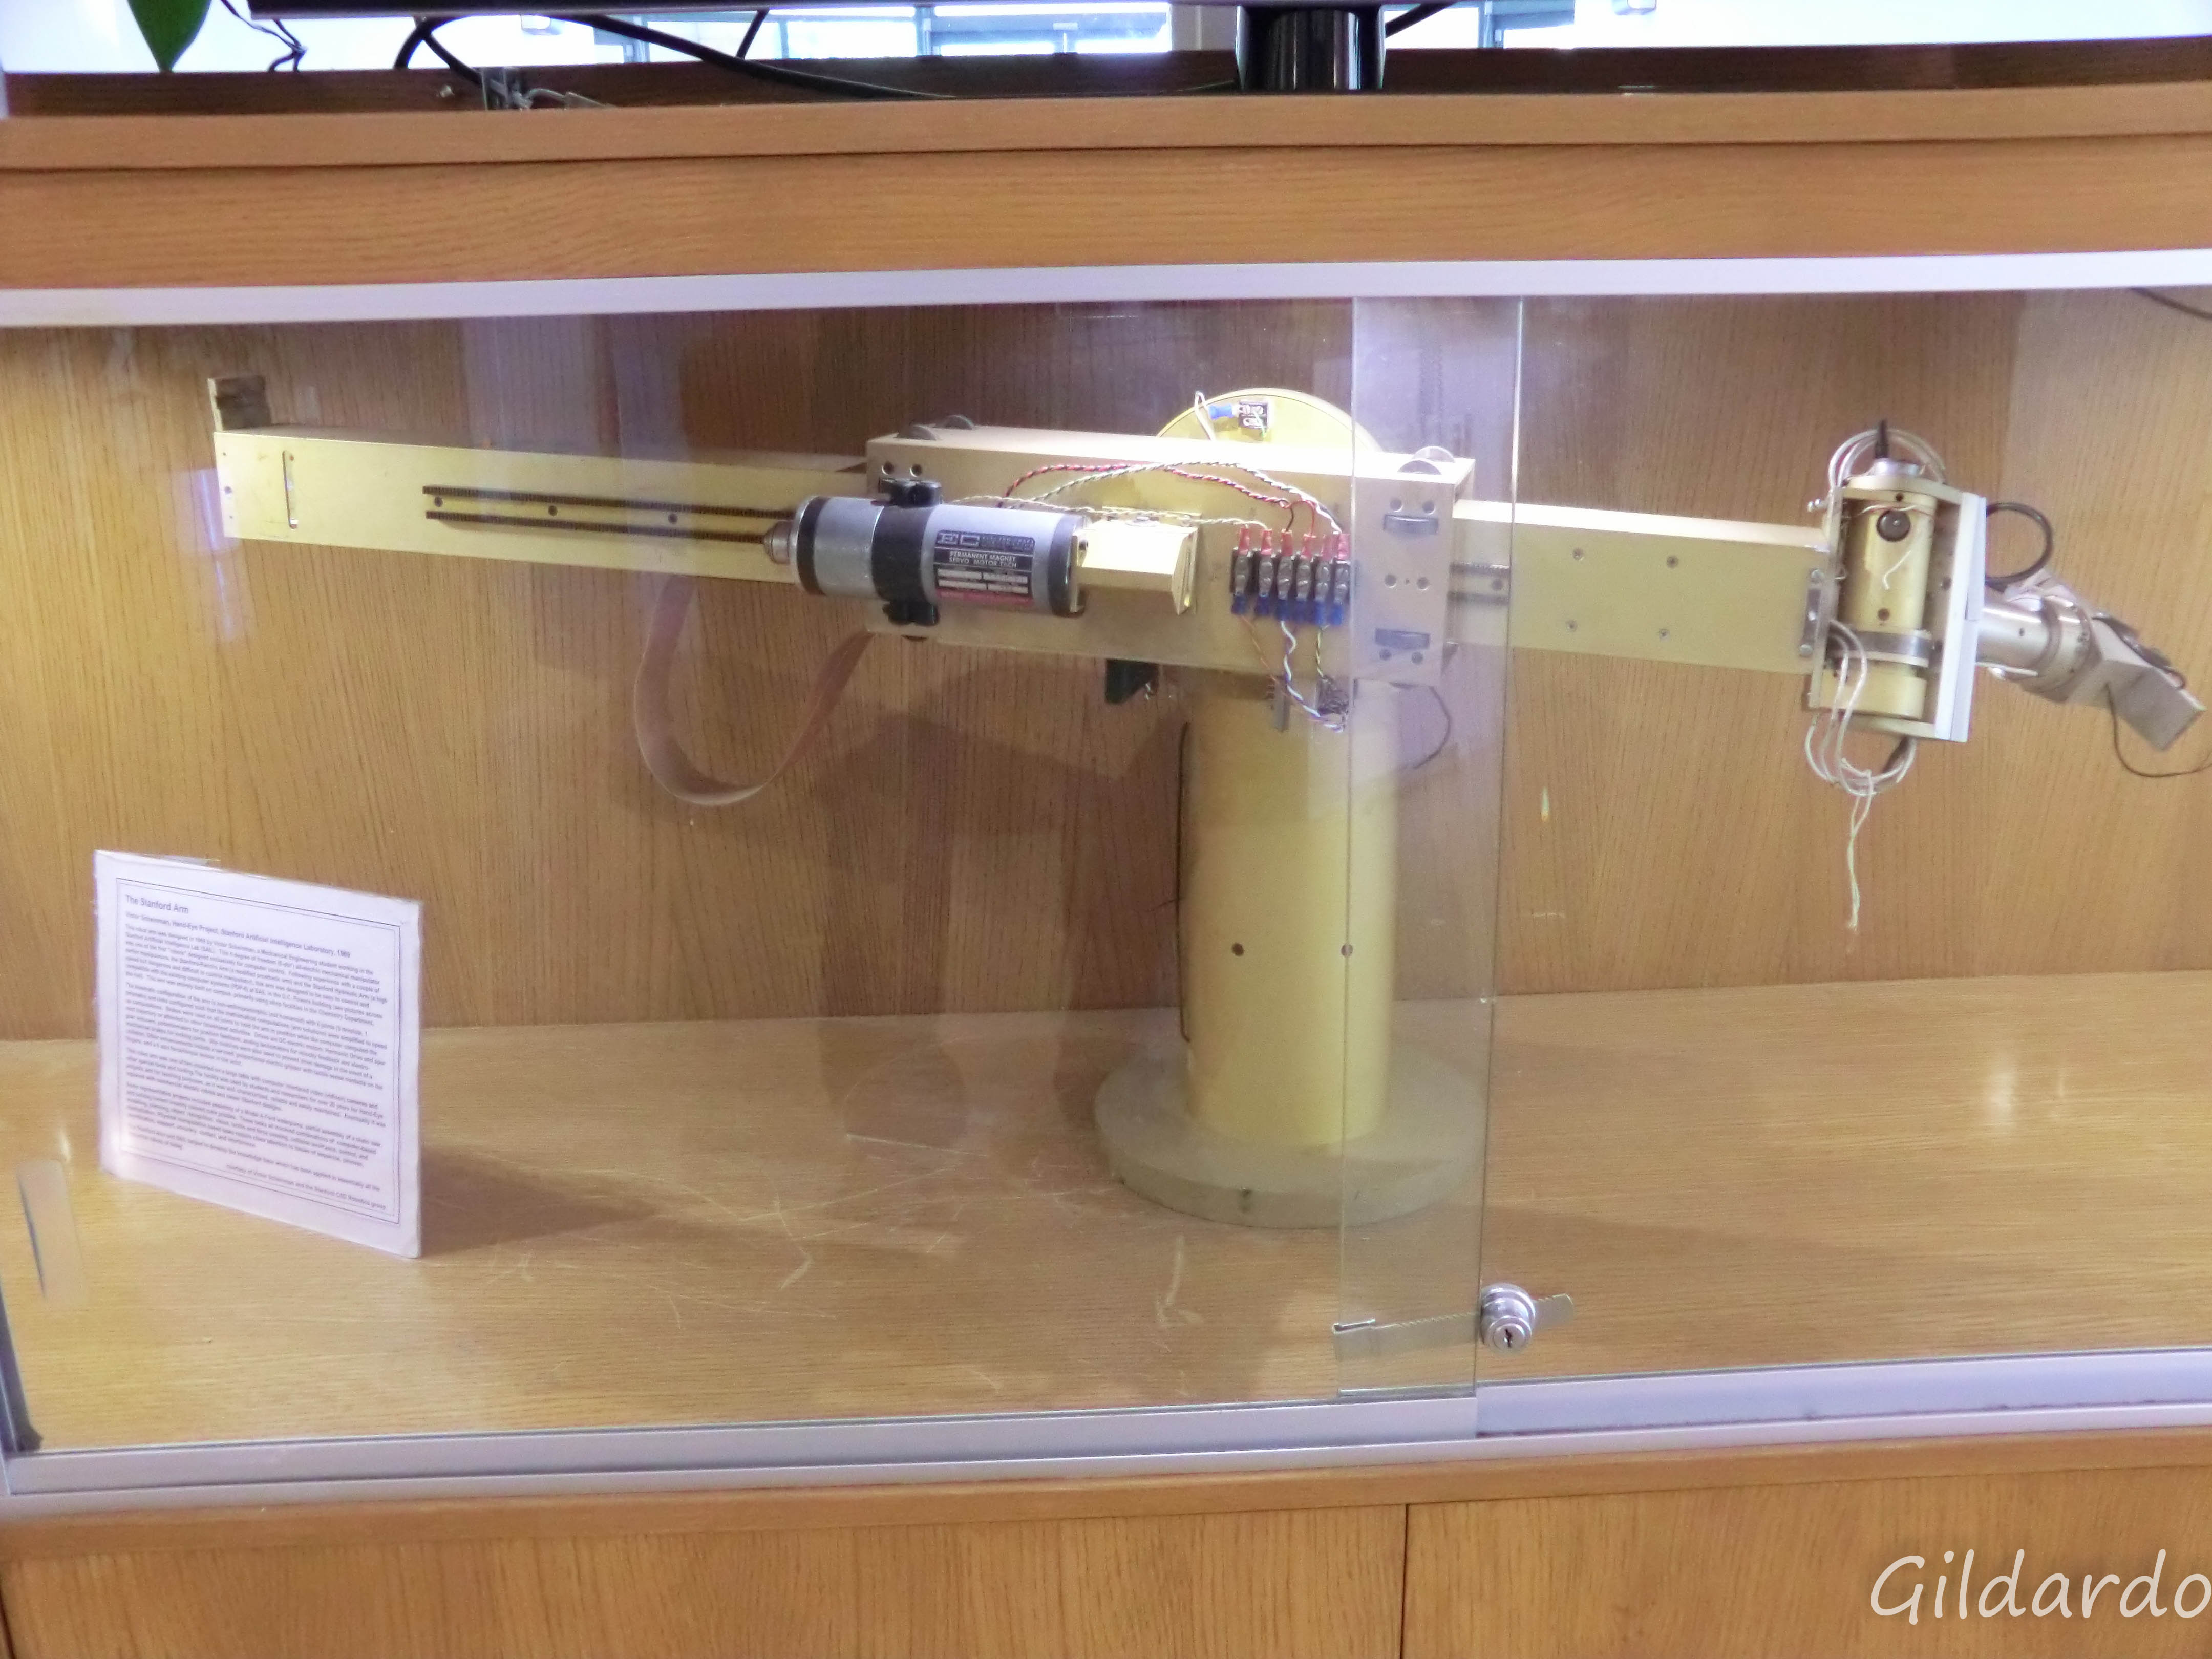
\includegraphics[scale=0.3]{./EtapaModerna/Imagenes/stanford_arm.jpg}
	\caption{Stanford Arm}
	\label{fig:stanfordArm}
\end{figure}

\subsubsection{T3}

Tras los grandes avances del Stanford Arm la compañía Cincinnati Milacron Corp. decidió desarrollar en 1973 el primer brazo robótico pensado para ser incorporado dentro del mercado industrial. El encargado dentro de la compañía de elaborar el diseño del brazo fue Richard Hohn.

\vspace{10px}

Este brazo robótico, al igual que el Stanford Arm fue desarrollado con 6 grados de libertad permitiendo un amplio abanico de movimientos que el brazo podía hacer con bastante precisión.

\vspace{10px}

Este brazo ya no tenía que ser controlado directamente por un humano, si no que implementaba un módulo de decisiones y sensores capaz de saber si había completado una cierta tarea y tenía que realizar algún movimiento, por ejemplo coger un elemento de una cinta de transporte y moverlo.

\subsubsection{PUMA}

Tras el éxito de los diseños de Victor Scheinman en la Universidad de Stanford, la compañía General Motors se interesó en sus prototipos de brazos robóticos. Ante el incipiente mercado de estos robots las grandes compañías con un gran nivel de fábricas comenzaron a ver una utilidad en estos brazos, por lo que General Motors financió a Scheinman para que desarrollara el brazo robótico PUMA (Programmable Universal Machine for Assembly o Programmable Universal Manipulation Arm).

El brazo se comercializó en tres tamaños distintos con la intención de que unos levantasen más peso que otros. Todos los brazos tenían el mismo diseño y los mismos grados de libertad, por lo que los movimientos posibles eran iguales para todos los modelos. Los ángulos máximos de giro y rotación variaban entre modelos, ya que hay que pensar que estos fueron creados casi \textit{ad hoc} para las compañías. Además los modelos más grandes tenían unos movimientos mucho más lentos debido al peso que tenían que soportar y mover por el diseño tan grande que tenían para la época.

Este modelo fue fabricado por General Motors, Westinghouse Electric Corp., Staubli e incluso la división de robótica de Nokia. Fue un éxito fabricándose únicamente por Nokia unos 1500 brazos robóticos PUMA.

\subsubsection{MOGURA}

No solo se hicieron brazos robóticos convencionales siguiendo los diseños de Stanford, si no que también surgieron algunos intentos más novedosos como el brazo robótico MOGURA. Este brazo surge como un diseño del profesor Shigeo Hirose, del Instituto Tecnológico de Tokyo. El profesor Hirose estaba estudiando robots que imitaran el comportamiento de animales, como por ejemplo las serpientes, con las que ideó un robot llamado ACMVI que imitaba el comportamiento de las mismas. De las articulaciones que desarrolló para este robot surgió la idea de hacer un brazo con más movilidad aún al que llamó MOGURA entorno al año 1978. Este brazo no tuvo un éxito muy destacable, ya que los diseños anteriores aún funcionaban bien y los siguientes intentos como SCARA cumplieron su función muy notablemente.

\subsubsection{SCARA}
Un avance muy grande en el ámbito de los brazos robóticos fueron los brazos SCARA (Selective Compliance Assembly Robot Arm o Selective Compliance Articulated Robot Arm). Estos brazos rompían la estructura de los antiguos diseños haciendo que la movilidad de los mismos fuera muy superior con movimientos mucho más rápidos. Estos robots fueron conceptualizados por las compañías Japonesas Sankyo Seiki, Pentel y NEC y fueron elaborados bajo la supervisión de Hiroshi Makino, un profesor de la Universidad de Yamanashi.

El diseño de este tipo de brazos pasaba de un robot que se movía únicamente como los ejes cartesianos, es decir en movimientos rectos muy fijos, a un movimiento muy ágil con ejes paralelos. El brazo SCARA se movía igual que los anteriores cartesianos, es decir, de forma recta con respecto a los ejes X,Y y Z pero además incluía un ángulo de giro en el plano del eje Z de forma que podía rotar las piezas que cogía.

Este tipo de robots son extremadamente útiles en la manipulación entre elementos en líneas de trabajo de fábricas, ya que con ellos se hace muy sencillo transportar objetos entre distintas fases en el proceso de un objeto. Por ejemplo podemos imaginar una línea de trabajo en la que se hacen puertas para vehículos, este robot podría transportar la puerta ya finalizada de la línea de fabricación de puertas, rotarla convenientemente y desplazarla hacia la línea de ensamblaje en el chasis del coche, de forma que movería la puerta él solo y el operario sólo tendría que atornillarla o realizar el ensamblaje que corresponda. Estos robots, gracias al ángulo de giro en el eje Z, pueden servir por ejemplo para atornillar piezas en una placa que se les coloque en la línea de ensamblaje tales como por ejemplo los tornillos que fijan ciertos componentes a la placa base de un móvil u ordenador.

Estos brazos robóticos supusieron un avance muy notable en su creación siendo incluso utilizados actualmente. Hay que tener en cuenta que los brazos robóticos siguen aún en desarrollo y casi a diario obtenemos nuevas mejoras en los mismos, pero estos fueron los que sentaron precedentes en lo que actualmente conocemos y asociamos con brazos robóticos.
